\chapter[Part 1]{}
\section{Company Profile}
FOREST Business Furniture is a renowned provider of bespoke commercial furniture
solutions, combining craftsmanship and innovation to create exceptional workspaces.
With a commitment to quality, design, and customer satisfaction,
we specialize in transforming office environments into functional and aesthetically
pleasing spaces that inspire productivity and collaboration.


Founded in 2010 by visionary furniture designer Polar Kaung, FOREST Business Furniture began as a small woodworking workshop in a queint town.
Polar's passion for blending natural elements with functional design has led to the company's rapid growth and reputation for producing unique and high-quality pieces.
Over the years, the company expanded its team of skilled craftsmen, embraced modern technology, and earned recognition for its innovative approach to office furniture.

\subsection{Organization Structure}
\begin{figure}[!h]
    \centering
    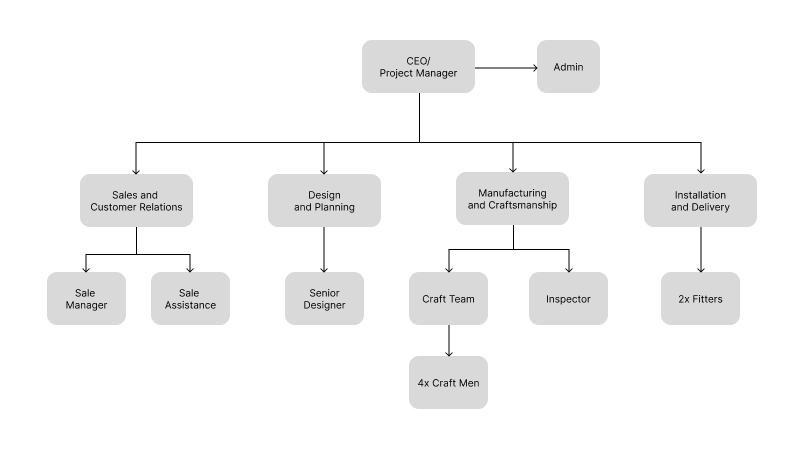
\includegraphics[scale=0.5]{Organization Structure.png}
    \caption{Organization Structure}
    \label{figure:organization_structure}
\end{figure}
In the organizational chart described in Figure \ref{figure:organization_structure}, 12 employees work under
 four teams. The four teams
are sales and customer relations team, design and planning team, manufacturing and craftsmanship team 
and installation and delivery team. 
Aside from four team there will be an admin that will work along side all teams.
Firstly, the
responsibility of sales team is to make advertisements for increasing the sales and getting
the customer. Next, they receive customer contact, make an appointment with customer
for order specifications. They handle project contract and arrange payment with customer.
And when the production is completed, they ask customer when to install and deliver.


The design team works together with the customer, sales team and admin for producing estimated quotation and finished time. 
They have responsibilities
for designing products with the customer's demands and confirming update the materials
price and delivery time. Then, they finally calculate the final cost and finished time after
considering all things in the project.


After receiving the order confirmation from customer, the production team starts to
purchase the materials. When the materials arrive, the production process starts. In the
production team, there are four multi-skilled crafts people who are able to manufacture all
types of furniture's. In those four craftsmen, there are one inspector who eventually check
the quality control and quality assurances. After inspecting all the products, they start to
pack the order. The installation team works when the customer confirms the date to deliver
and install.
\newpage
\subsection{Vision}
The vision of FOREST Business Furniture is to create imaginative, custom-made furniture solutions that transform tired work settings into inspiring environments. We aim to lead the industry by seamlessly merging great craftsmanship, functionality, and aesthetics to develop furniture that not only meets the needs of our clients but also improves their work experience. Our commitment to excellence, sustainability, and personalized service drives us to consistently offer furniture that inspires creativity. Our mission stays the same as we grow: to determine the future of work environments by rethinking furniture design and setting new quality and innovation standards.
\subsection{Mission}
Our goal at FOREST Business Furniture is to create, assemble, and distribute office furniture that makes ordinary rooms into exceptional workspaces. We are dedicated to offering our clients professionally created and unique furniture options that suit their practical requirements and enhance wellbeing. We try to produce furniture items that are a tribute to our unrelenting quest of perfection, with a focus on innovation, sustainability, and high-caliber craftsmanship. We are motivated to constantly push the frontiers of creativity and usefulness because we have a keen knowledge of the tremendous effects that a well-designed workstation can have on individuals and teams.
\newpage
\section{Business Case}
The company follows a straightforward sequential approach in its operations.
It all begins with customers reaching out to a sales representative through phone calls, the company's website, or interactions at sales events.
Once an inquiry is made, a sales team member and an admin arrange a meeting with the customer to define the order specifications. Collaborating with the design team, the sales team then creates a quotation. Using the order specifications, the design team generates designs for tables and chairs, along with installation layouts.

The company's designers and sales team assess the order to generate an estimate, which is communicated to the customer. After finalizing the design, the craftsmen commence production, considering the company's overall production capacity. The production process kicks off by coordinating with material suppliers and procuring the necessary materials beforehand.

Next, the Quality Assurance and Quality Control team examines the products, issuing a Change Order for any faulty items. Following successful QA/QC inspection, the products undergo packing and shipping. Upon arrival at the customer's location, the items are installed by the company's installers. As part of our commitment to maintaining strong customer relationships, we offer after-sales support and reasonably priced repair services for our products within a six-month timeframe.
\subsection{IDEF (A-0) Diagram}
The IDEF0 A-0 (pronounced "A minus zero") diagram presents a context-level
view of the inputs, control, outputs, and mechanisms (ICOM) for a specific function in
your logical model. DEF0 stands for Integration Definition for Process Modelling, a
public-domain methodology used to model businesses and their processes so they
can be understood and improved.
The IDEF (A-0) parent diagram of Forest Business Design manufacture
process is defined in Figure \ref{figure:idef_a_0}
\begin{figure}[!h]
    \centering
    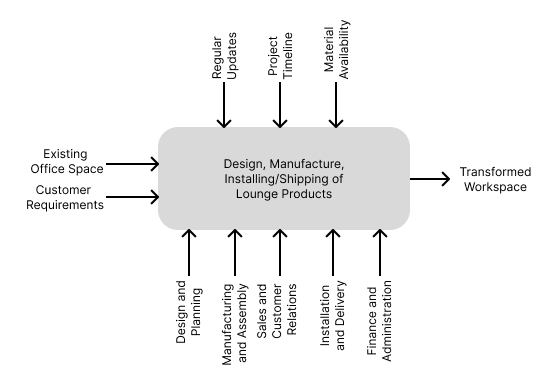
\includegraphics[scale=0.5]{IDEF (A-0).png}
    \caption{IDEF (A-0)}
    \label{figure:idef_a_0}
\end{figure}
\paragraph*{Purpuse:}
To illustrate IDEF0 modeling for the designing, manufacturing and installation processes of furniture
by the company.
\paragraph*{Context:}
The company has required technical knowledge and skilled craftsmen to
carry out the manufacturing order and need not outsource them. All operation is
carried out by employees already hired by the company starting from receiving
customer enquiry to installation of the furniture at the client's place.
\paragraph*{Viewpoint}
The CEO The overlooks the whole operation of the company with the
approval of clients and Chief Executive Officer.
\subsection{IDEF0 Diagram}
\begin{figure}[!h]
    \centering
    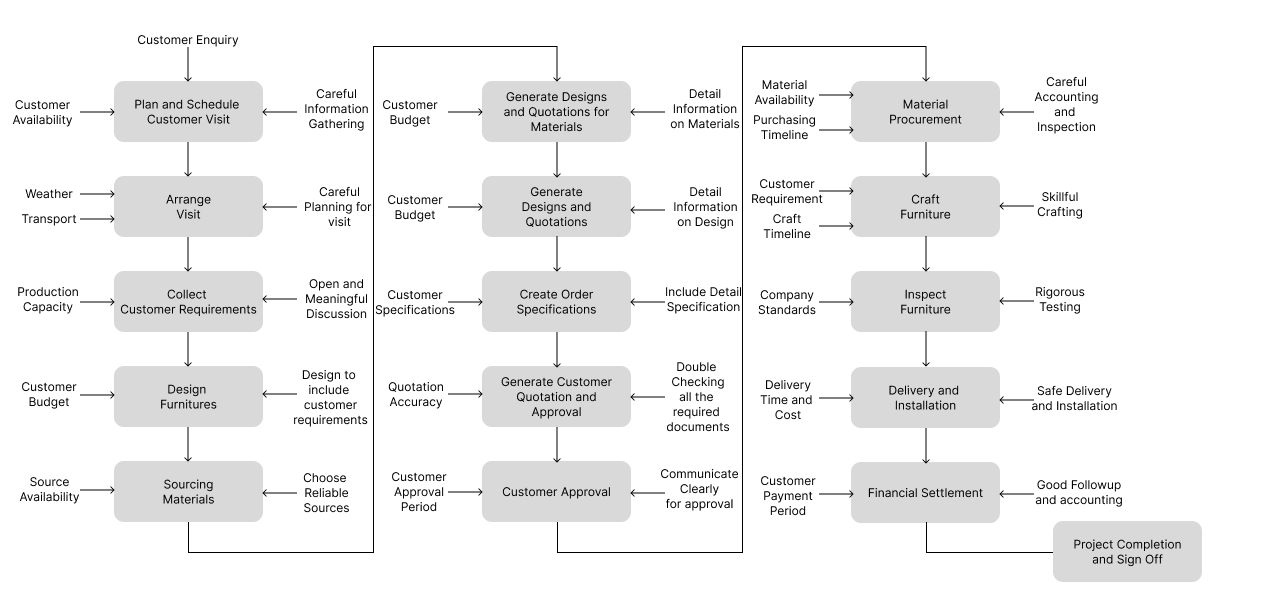
\includegraphics[scale=0.4,center]{Improved IDEF0.png}
    \caption{IDEF0}
    \label{figure:idef0}
\end{figure}
\newpage
\section{Appraisal or Evaluation and Summary}
In figure \ref{figure:idef0}, (IDEF0) model described step by step manufacturing process of
the company. The entire process starts with receiving customer inquiry. Once the
customer contacts to sale center, the clerk makes plans and arrange an appointment with sales team and
admin. The sales team collect the detail requirements for the project with the company capacity in mind.
Then, with the requirements, the design team starts designing along with the approximated materials required and sources.
After that, the design team generates quotations on materails and the overall designs, then create a detail order specifications.
Once this is done, the quotation for the custormer is made and inform the customer.
After getting agreement on the design and quotation, General manager calls the project
planning meeting to make step by step project plan creating work break down
structure, project schedule, Gantt chart, project risks register, etc. The manufacturing
process require involvement of the material suppliers. Design engineers start to design
furniture depending on project specifications following the quality standard. After
design is finished, craftsmen start to build furniture. During building the furniture,
carpenters and staffs need to wear safety suit and helmet because safety is the
biggest concern of the company.
After building the designed furniture, quality control team will check the built
furniture which meets customer expectation. Installation process will start after
checking the built furniture and deliver the products to customer. In case the products
undergo some faults in the process of manufacturing, our company gives full
repairment free to customers with the aid of after sales service team.
There might be a few changes here and there which can easily be adjusted in
this model. For example, the customer might not always want to visit the firm,
especially the repeated customers. Additionally, in case of repeated orders, the firms
may also not follow the usual process of redesigning the items again and again unless
there are important changes. The model shows flexibility as these steps can be
omitted in the working of the firm. Instead the process follows the same route and
nothing changes besides these omissions.
\end{enumerate}